\section{Database Management}

A database is an efficient and well organized method of storing and accessing the statistics collected by the system nodes. A MySQL database was selected for it's clear documentation and easy integration into Python applications via the MySQLConnector class \cite{mysqlconnector}. A single database maintained on a machine on the same network as the nodes is used to store the statistics they transmit. The design of the system can be seen in Figure \ref{fig:erd} and Table \ref{table:entity_attributes} and as can be seen the database is relatively simple with only three entity types. The node entity represents a node in the monitoring system and stores the information important for identifying and locating it. The speed and count record entities each belong to a specific node and have a timestamp, an instance of these records is created every 30 seconds for a node. For a count record the vehicle count for the 30 seconds passed is stored and for the a speed record the average speed for that last 30 seconds is stored. If data needs to be consolidated into different time scales individual 30 second readings are summed and served up by the server-side logic, a small library was written to this end that takes a time range and returns readings from this range compressed into a desired time period. 

\begin{figure}[H]
    \centering
    \centering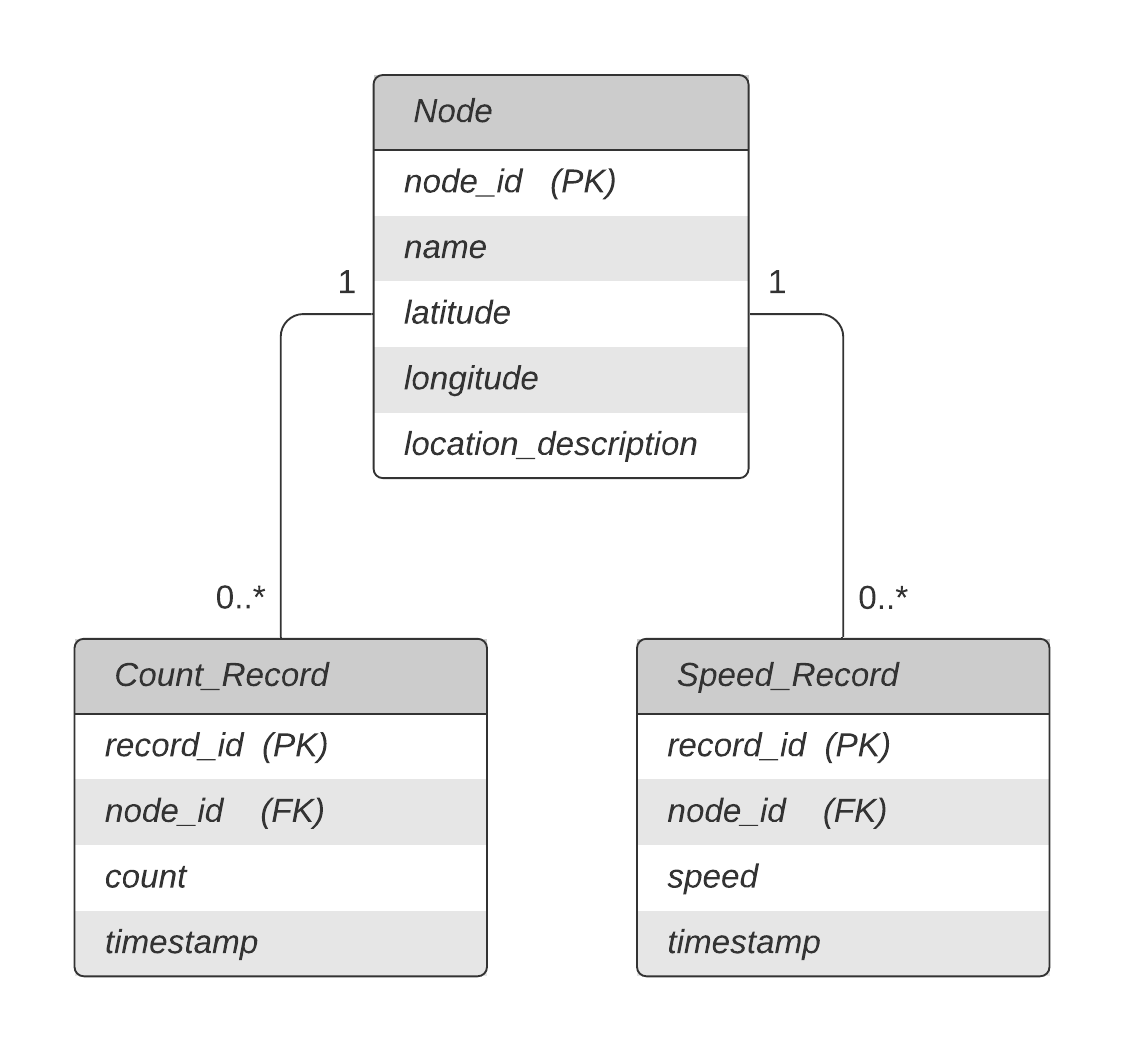
\includegraphics[width = 0.8\textwidth]{design/database/dragonfly_database_ERD}
    \caption{Entity Relationship Diagram of the system database.}
    \label{fig:erd}
  \end{figure}

\begin{table}
\def\arraystretch{1.5}
\begin{center}
\begin{singlespace}
    \begin{tabular}{|M{2.5cm}|M{2cm}|M{4cm}|M{3cm}|M{1cm}|} 
        \hline
        \textbf{Entity Name} & \textbf{Attributes} & \textbf{Description} & \textbf{Data Type} & \textbf{Null}\\
        \hline
        \multirow{5}{*}{Node} 
        & node id & A number that uniquely identifies the entity. & INT & N\\ \cline{2-5}
        & latitude & Latitude used to locate node. & DECIMAL(10,8) & N\\ \cline{2-5}
        & longitude & Longitude used to locate node. & DECIMAL(10,8) & N\\ \cline{2-5}
        & location description & Information helpful when locating the node in addition to its longitude and latitude. & VARCHAR(120) & Y\\
        \hhline{|=|=|=|=|=|}
        \multirow{5}{*}{Speed Record} 
        & record id & A number that uniquely identifies the entity. & INT & N\\ \cline{2-5}
        & node id & Unique node identifier linking record to its node. & INT & N\\ \cline{2-5}
        & speed & A single speed reading averaging vehicle speeds over 30 seconds. & DECIMAL(4,2) & N\\ \cline{2-5}
        & timestamp & Time stamp indicating when the speed reading began collecting data. & DATETIME & N\\
        \hhline{|=|=|=|=|=|}
        \multirow{5}{*}{Count Record} 
        & record id & A number that uniquely identifies the entity. & INT & N\\ \cline{2-5}
        & node id & Unique node identifier linking record to its node. & INT & N\\ \cline{2-5}
        & count & A single count reading for 30 seconds of traffic. & DECIMAL(4,2) & N\\ \cline{2-5}
        & timestamp & Time stamp indicating when the speed reading began collecting data. & DATETIME & N\\
        \hline
    \end{tabular}
\end{singlespace}
\end{center}
\caption{Attribute data for the system's database entities.}
\label{table:entity_attributes}
\end{table}